\section{Split-Transaction Bus, case of the MSI Protocol}
\label{sec:split_msi}
Section~\ref{sec:intro_to_msi} provides an overview of the MSI protocol without
considerations for the possibility of interleaving or even asynchronous
communications. This section presents an MSI protocol featuring all of those.
This leads a large number of additional states and transitions, so instead of
using graphs to represent the automata, we use matrices (see
Figure~\ref{fig:msi_cc_table} for the cache controllers, and
Figure~\ref{fig:msi_mgr_table} for the coherence manager). The columns in
these matrices correspond to the events from Definition~\ref{def:event}. Bear
in mind that this corresponds to how the caches and the coherence manager act
for each memory element, according to the state currently assigned to that
state (first column). The \textbf{Own Query} column in the cache's
table corresponds to when it processes one of its own queries (from its incoming
query queue) for that memory element. In the coherence manager's table, the
behavior upon reception of a query may differ according to whether the emitter
is the owner (as defined by the \coherencemanagerownerfun{} function) or not.

\subsection{State Naming}
\label{sec:cache_state_naming}
Invalid (\texttt{I}), Shared (\texttt{S}), and Modified (\texttt{M}) are the
three stable states of the \texttt{MSI} protocol, the other states are
transient.

Reception of a request that requires use of the interconnect will usually lead
to a \texttt{XY\textsuperscript{BD}} transient state, which means that the
cache controller is handling a transition between the stable states \texttt{X}
and \texttt{Y}, with \textsuperscript{B} indicating that this transition
requires the acquisition of the interconnect and \textsuperscript{D} the
reception of a related data reply (regardless of whether it comes from an other
cache controller or the memory).

\texttt{XY\textsuperscript{D}} usually follows \texttt{XY\textsuperscript{BD}}
if the cache controller sees its own query before receiving a reply. If the
reply is seen first, then the memory element goes into the
\texttt{XY\textsuperscript{B}} state instead. While the former is more likely,
the latter may occur because, despite processing all queries in the same order,
not all cache controllers take the same time to do so.

It is also possible an external query to lead to a change of state, especially
when in the \texttt{XY\textsuperscript{D}} state. Indeed, at that point, the
system pretty much considers that the cache controller is in the \texttt{Y}
state, and thus has the responsibilities that the \texttt{Y} state would imply.
This makes it possible for a cache controller to see a query it needs to act
upon before being actually ready to do so (e.g.~observing a \texttt{GetM} query
while waiting for \texttt{data}). The states thus reached have either a
\texttt{XY\textsuperscript{D}V} pattern, with \texttt{V} being a stable state,
indicating that the external query would have required this memory element to be
assigned the \texttt{V} state if it were currently in the \texttt{Y} state.
Thus, this state is used to memorize that, after sending the data, the cache is
expected to perform the appropriate change of state. It is possible for
the \texttt{Y} state to also be susceptible to external queries. Thus, there
are also \texttt{XY\textsuperscript{D}YZ} states, indicating that the final
state is now \texttt{Z}.

\begin{figure}
\begin{center}
\begin{tabular}{|l||c|c|c|c|c||c|c|c|}
 \hline

 \textbf{State}
 & \multicolumn{3}{c|}{\textbf{Core Request}}
 & \begin{tabular}{@{}c@{}}
      \textbf{Own}\\
      \textbf{Query}
   \end{tabular}
 & \begin{tabular}{@{}c@{}}
      \textbf{Data}\\
      \textbf{Reply}
   \end{tabular}
 & \multicolumn{3}{c|}{\textbf{Received Queries}}
 \\

%%%%%%%%%%%%%%%%%%%%%%%%%%%%%%%%%%%%%%%%%%%%%%%%%%%%%%%%%%%%%%%%%%%%%%%%%%%%%%%%
 & \loadinstr{} & \storeinstr{} & \evictinstr{}
 &
 &
 & \getsquery{} & \getmquery{} & \putmquery{}
 \\
 \hline

%%%%%%%%%%%%%%%%%%%%%%%%%%%%%%%%%%%%%%%%%%%%%%%%%%%%%%%%%%%%%%%%%%%%%%%%%%%%%%%%
 \texttt{I}

 % Load/Store/Evict
 &
   \begin{tabular}{@{}c@{}}
      \sendqueryact{\getsquery{}}\\
      \setstateact{\texttt{IS\textsuperscript{BD}}}
   \end{tabular}
 &
   \begin{tabular}{@{}c@{}}
      \sendqueryact{\getmquery{}}\\
      \setstateact{\texttt{IM\textsuperscript{BD}}}
   \end{tabular}
 & \disablecell{}

 % Seeing Own Query
 & \disablecell{}

 % Data Reply
 & \disablecell{}

 % GetS/GetM/PutM
 & \noaction{}
 & \noaction{}
 & \noaction{}
 \\
 \hline

%%%%%%%%%%%%%%%%%%%%%%%%%%%%%%%%%%%%%%%%%%%%%%%%%%%%%%%%%%%%%%%%%%%%%%%%%%%%%%%%
 \texttt{IS\textsuperscript{BD}}

 % Load/Store/Evict
 & \stallact{}
 & \stallact{}
 & \stallact{}

 % Seeing Own Query
 & \setstateact{\texttt{IS\textsuperscript{D}}}

 % Data Reply
 & \setstateact{\texttt{IS\textsuperscript{B}}}

 % GetS/GetM/PutM
 & \noaction{}
 & \noaction{}
 & \noaction{}
 \\
 \hline

%%%%%%%%%%%%%%%%%%%%%%%%%%%%%%%%%%%%%%%%%%%%%%%%%%%%%%%%%%%%%%%%%%%%%%%%%%%%%%%%
 \texttt{IS\textsuperscript{B}}

 % Load/Store/Evict
 & \stallact{}
 & \stallact{}
 & \stallact{}

 % Seeing Own Query
 & \setstateact{\texttt{S}}

 % Data Reply
 & \disablecell{}

 % GetS/GetM/PutM
 & \noaction{}
 & \noaction
 & \disablecell{}
 \\
 \hline

%%%%%%%%%%%%%%%%%%%%%%%%%%%%%%%%%%%%%%%%%%%%%%%%%%%%%%%%%%%%%%%%%%%%%%%%%%%%%%%%
 \texttt{IS\textsuperscript{D}}

 % Load/Store/Evict
 & \stallact{}
 & \stallact{}
 & \stallact{}

 % Seeing Own Query
 & \disablecell{}

 % Data Reply
 & \setstateact{\texttt{S}}

 % GetS/GetM/PutM
 & \noaction{}
 & \setstateact{\texttt{IS\textsuperscript{D}I}}
 & \disablecell{}
 \\
 \hline

%%%%%%%%%%%%%%%%%%%%%%%%%%%%%%%%%%%%%%%%%%%%%%%%%%%%%%%%%%%%%%%%%%%%%%%%%%%%%%%%
 \texttt{IS\textsuperscript{D}I}

 % Load/Store/Evict
 & \stallact{}
 & \stallact{}
 & \stallact{}

 % Seeing Own Query
 & \disablecell{}

 % Data Reply
 & \setstateact{\texttt{I}}

 % GetS/GetM/PutM
 & \noaction{}
 & \noaction{}
 & \disablecell{}
 \\
 \hline

%%%%%%%%%%%%%%%%%%%%%%%%%%%%%%%%%%%%%%%%%%%%%%%%%%%%%%%%%%%%%%%%%%%%%%%%%%%%%%%%
 \texttt{IM\textsuperscript{BD}}

 % Load/Store/Evict
 & \stallact{}
 & \stallact{}
 & \stallact{}

 % Seeing Own Query
 & \setstateact{\texttt{IM\textsuperscript{D}}}

 % Data Reply
 & \setstateact{\texttt{IM\textsuperscript{B}}}

 % GetS/GetM/PutM
 & \noaction{}
 & \noaction{}
 & \noaction{}
 \\
 \hline

%%%%%%%%%%%%%%%%%%%%%%%%%%%%%%%%%%%%%%%%%%%%%%%%%%%%%%%%%%%%%%%%%%%%%%%%%%%%%%%%
 \texttt{IM\textsuperscript{B}}

 % Load/Store/Evict
 & \stallact{}
 & \stallact{}
 & \stallact{}

 % Seeing Own Query
 & \setstateact{\texttt{M}}

 % Data Reply
 & \disablecell{}

 % GetS/GetM/PutM
 & \noaction{}
 & \noaction{}
 & \noaction{}
 \\
 \hline

%%%%%%%%%%%%%%%%%%%%%%%%%%%%%%%%%%%%%%%%%%%%%%%%%%%%%%%%%%%%%%%%%%%%%%%%%%%%%%%%
 \texttt{IM\textsuperscript{D}}

 % Load/Store/Evict
 & \stallact{}
 & \stallact{}
 & \stallact{}

 % Seeing Own Query
 & \disablecell{}

 % Data Reply
 & \setstateact{\texttt{M}}

 % GetS/GetM/PutM
 & \begin{tabular}{@{}c@{}}
      \storereplytoact{}\\
      \setstateact{\texttt{IM\textsuperscript{D}S}}
   \end{tabular}
 & \begin{tabular}{@{}c@{}}
      \storereplytoact{}\\
      \setstateact{\texttt{IM\textsuperscript{D}I}}
   \end{tabular}
 & \disablecell{}
 \\
 \hline

%%%%%%%%%%%%%%%%%%%%%%%%%%%%%%%%%%%%%%%%%%%%%%%%%%%%%%%%%%%%%%%%%%%%%%%%%%%%%%%%
 \texttt{IM\textsuperscript{D}I}

 % Load/Store/Evict
 & \stallact{}
 & \stallact{}
 & \stallact{}

 % Seeing Own Query
 & \disablecell{}

 % Data Reply
 &
   \begin{tabular}{@{}c@{}}
      \senddataact{\replytotarget{}}{\simpledata{}}\\
      \setstateact{\texttt{I}}
   \end{tabular}

 % GetS/GetM/PutM
 & \noaction{}
 & \noaction{}
 & \disablecell{}
 \\
 \hline

%%%%%%%%%%%%%%%%%%%%%%%%%%%%%%%%%%%%%%%%%%%%%%%%%%%%%%%%%%%%%%%%%%%%%%%%%%%%%%%%
 \texttt{IM\textsuperscript{D}S}

 % Load/Store/Evict
 & \stallact{}
 & \stallact{}
 & \stallact{}

 % Seeing Own Query
 & \disablecell{}

 % Data Reply
 & \begin{tabular}{@{}c@{}}
      \senddataact{\replytotarget{}}{\simpledata{}}\\
      \senddataact{\memorytarget{}}{\simpledata{}}\\
      \setstateact{\texttt{I}}
   \end{tabular}

 % GetS/GetM/PutM
 & \noaction{}
 & \setstateact{\texttt{IM\textsuperscript{D}SI}}
 & \disablecell{}
 \\
 \hline

%%%%%%%%%%%%%%%%%%%%%%%%%%%%%%%%%%%%%%%%%%%%%%%%%%%%%%%%%%%%%%%%%%%%%%%%%%%%%%%%
 \texttt{IM\textsuperscript{D}SI}

 % Load/Store/Evict
 & \stallact{}
 & \stallact{}
 & \stallact{}

 % Seeing Own Query
 & \disablecell{}

 % Data Reply
 & \begin{tabular}{@{}c@{}}
      \senddataact{\replytotarget{}}{\simpledata{}}\\
      \senddataact{\memorytarget{}}{\simpledata{}}\\
      \setstateact{\texttt{I}}
   \end{tabular}

 % GetS/GetM/PutM
 & \noaction{}
 & \noaction{}
 & \disablecell{}
 \\
 \hline

%%%%%%%%%%%%%%%%%%%%%%%%%%%%%%%%%%%%%%%%%%%%%%%%%%%%%%%%%%%%%%%%%%%%%%%%%%%%%%%%
 \texttt{S}

 % Load/Store/Evict
 & \hitact{}
 &
   \begin{tabular}{@{}c@{}}
      \sendqueryact{\getmquery{}}\\
      \setstateact{\texttt{SM\textsuperscript{BD}}}
   \end{tabular}
 & \setstateact{\texttt{I}}

 % Seeing Own Query
 & \disablecell{}

 % Data Reply
 & \disablecell{}

 % GetS/GetM/PutM
 & \noaction{}
 & \setstateact{\texttt{I}}
 & \disablecell{}
 \\
 \hline

%%%%%%%%%%%%%%%%%%%%%%%%%%%%%%%%%%%%%%%%%%%%%%%%%%%%%%%%%%%%%%%%%%%%%%%%%%%%%%%%
 \texttt{SM\textsuperscript{BD}}

 % Load/Store/Evict
 & \hitact{}
 & \stallact{}
 & \stallact{}

 % Seeing Own Query
 & \setstateact{\texttt{SM\textsuperscript{D}}}

 % Data Reply
 & \setstateact{\texttt{SM\textsuperscript{B}}}

 % GetS/GetM/PutM
 & \noaction{}
 & \setstateact{\texttt{IM\textsuperscript{BD}}}
 & \disablecell{}
 \\
 \hline

%%%%%%%%%%%%%%%%%%%%%%%%%%%%%%%%%%%%%%%%%%%%%%%%%%%%%%%%%%%%%%%%%%%%%%%%%%%%%%%%
 \texttt{SM\textsuperscript{B}}

 % Load/Store/Evict
 & \hitact{}
 & \stallact{}
 & \stallact{}

 % Seeing Own Query
 & \setstateact{\texttt{M}}

 % Data Reply
 & \disablecell{}

 % GetS/GetM/PutM
 & \noaction{}
 & \setstateact{\texttt{IM\textsuperscript{B}}}
 & \disablecell{}
 \\
 \hline


%%%%%%%%%%%%%%%%%%%%%%%%%%%%%%%%%%%%%%%%%%%%%%%%%%%%%%%%%%%%%%%%%%%%%%%%%%%%%%%%
 \texttt{SM\textsuperscript{D}}

 % Load/Store/Evict
 & \hitact{}
 & \stallact{}
 & \stallact{}

 % Seeing Own Query
 & \disablecell{}

 % Data Reply
 & \setstateact{\texttt{M}}

 % GetS/GetM/PutM
 & \begin{tabular}{@{}c@{}}
      \senddataact{\replytotarget{}}{\simpledata{}}\\
      \setstateact{\texttt{SM\textsuperscript{D}S}}
   \end{tabular}
 & \begin{tabular}{@{}c@{}}
      \senddataact{\replytotarget{}}{\simpledata{}}\\
      \setstateact{\texttt{SM\textsuperscript{D}I}}
   \end{tabular}
 & \disablecell{}
 \\
 \hline

%%%%%%%%%%%%%%%%%%%%%%%%%%%%%%%%%%%%%%%%%%%%%%%%%%%%%%%%%%%%%%%%%%%%%%%%%%%%%%%%
 \texttt{SM\textsuperscript{D}I}

 % Load/Store/Evict
 & \hitact{}
 & \stallact{}
 & \stallact{}

 % Seeing Own Query
 & \disablecell{}

 % Data Reply
 & \begin{tabular}{@{}c@{}}
      \senddataact{\replytotarget{}}{\simpledata{}}\\
      \setstateact{\texttt{I}}
   \end{tabular}

 % GetS/GetM/PutM
 & \noaction{}
 & \noaction{}
 & \disablecell{}
 \\
 \hline

%%%%%%%%%%%%%%%%%%%%%%%%%%%%%%%%%%%%%%%%%%%%%%%%%%%%%%%%%%%%%%%%%%%%%%%%%%%%%%%%
 \texttt{SM\textsuperscript{D}S}

 % Load/Store/Evict
 & \hitact{}
 & \stallact{}
 & \stallact{}

 % Seeing Own Query
 & \disablecell{}

 % Data Reply
 & \begin{tabular}{@{}c@{}}
      \senddataact{\replytotarget{}}{\simpledata{}}\\
      \senddataact{\memorytarget{}}{\simpledata{}}\\
      \setstateact{\texttt{S}}
   \end{tabular}

 % GetS/GetM/PutM
 & \noaction{}
 & \setstateact{\texttt{SM\textsuperscript{D}SI}}
 & \disablecell{}
 \\
 \hline

%%%%%%%%%%%%%%%%%%%%%%%%%%%%%%%%%%%%%%%%%%%%%%%%%%%%%%%%%%%%%%%%%%%%%%%%%%%%%%%%
 \texttt{SM\textsuperscript{D}SI}

 % Load/Store/Evict
 & \hitact{}
 & \stallact{}
 & \stallact{}

 % Seeing Own Query
 & \disablecell{}

 % Data Reply
 & \begin{tabular}{@{}c@{}}
      \senddataact{\replytotarget{}}{\simpledata{}}\\
      \senddataact{\memorytarget{}}{\simpledata{}}\\
      \setstateact{\texttt{I}}
   \end{tabular}

 % GetS/GetM/PutM
 & \noaction{}
 & \noaction{}
 & \disablecell{}
 \\
 \hline

%%%%%%%%%%%%%%%%%%%%%%%%%%%%%%%%%%%%%%%%%%%%%%%%%%%%%%%%%%%%%%%%%%%%%%%%%%%%%%%%
 \texttt{M}

 % Load/Store/Evict
 & \hitact{}
 & \hitact{}
 & \begin{tabular}{@{}c@{}}
      \sendqueryact{\putmquery{}}\\
      \setstateact{\texttt{MI\textsuperscript{B}}}
   \end{tabular}

 % Seeing Own Query
 & \disablecell{}

 % Data Reply
 & \disablecell{}

 % GetS/GetM/PutM
 &
   \begin{tabular}{@{}c@{}}
      \senddataact{\memorytarget{}}{\simpledata{}}\\
      \senddataact{\sendertarget{}}{\simpledata{}}\\
      \setstateact{\texttt{S}}
   \end{tabular}
 &
   \begin{tabular}{@{}c@{}}
      \senddataact{\sendertarget{}}{\simpledata{}}\\
      \setstateact{\texttt{I}}
   \end{tabular}
 & \disablecell{}
 \\
 \hline

%%%%%%%%%%%%%%%%%%%%%%%%%%%%%%%%%%%%%%%%%%%%%%%%%%%%%%%%%%%%%%%%%%%%%%%%%%%%%%%%
 \texttt{MI\textsuperscript{B}}

 % Load/Store/Evict
 & \hitact{}
 & \hitact{}
 & \stallact{}

 % Seeing Own Query
 &
   \begin{tabular}{@{}c@{}}
      \senddataact{\memorytarget{}}{\simpledata{}}\\
      \setstateact{\texttt{I}}
   \end{tabular}

 % Data Reply
 & \disablecell{}

 % GetS/GetM/PutM
 &
   \begin{tabular}{@{}c@{}}
      \senddataact{\memorytarget{}}{\simpledata{}}\\
      \senddataact{\sendertarget{}}{\simpledata{}}\\
      \setstateact{\texttt{II\textsuperscript{B}}}
   \end{tabular}
 &
   \begin{tabular}{@{}c@{}}
      \senddataact{\sendertarget{}}{\simpledata{}}\\
      \setstateact{\texttt{II\textsuperscript{B}}}
   \end{tabular}
 & \disablecell{}
 \\
 \hline

%%%%%%%%%%%%%%%%%%%%%%%%%%%%%%%%%%%%%%%%%%%%%%%%%%%%%%%%%%%%%%%%%%%%%%%%%%%%%%%%
 \texttt{II\textsuperscript{B}}

 % Load/Store/Evict
 & \stallact{}
 & \stallact{}
 & \stallact{}

 % Seeing Own Query
 & \setstateact{\texttt{I}}

 % Data Reply
 & \disablecell{}

 % GetS/GetM/PutM
 & \noaction{}
 & \noaction{}
 & \noaction{}
 \\
 \hline

 \multicolumn{1}{l|}{}
 & \multicolumn{5}{c||}{\textbf{Handling Requests}}
 & \multicolumn{3}{c|}{\textbf{Handling Queries}}
 \\
 \cline{2-9}
\end{tabular}

\end{center}
\caption{Split-Transaction MSI Automaton for Cache Controllers}
\label{fig:msi_cc_table}
\end{figure}
%
%Figure~\ref{fig:msi_mgr_table} shows how the coherency manager keeps track of
%whether the RAM has the most up-to-date value for a memory element (state
%\texttt{I}) or if a cache controller does (state \texttt{M}). This is used to
%determine if the RAM should be the one to reply when either a \texttt{GetS} or a
%\texttt{GetM} query passes through the interconnect. The \texttt{I} state
%indicates that the RAM currently has the most up-to-date value. The
%\texttt{I\textsuperscript{D}} state indicates that the RAM should be the one to
%respond to queries, but it still hasn't received the latest value.  Unlike the
%cache controller, it will not switch to a dedicated state but instead force
%queries from the interconnect to stall until the problematic query can be
%fulfilled. \texttt{I\textsuperscript{B}} indicates that the RAM has received
%the latest value, but has not yet seen the query that led this data to be sent.

\begin{figure}
\begin{center}
\input{\chapterdirectory/figure/split_msi_coherence_manager.tex}
\end{center}
\caption{Split-Transaction MSI Automaton for Coherence Manager}
\label{fig:msi_mgr_table}
\end{figure}

\stopallthesefloats
\subsection{Examples}
\stopallthesefloats
\begin{example}[Simple Read]
\label{ex:split_msi_simple_read}
In this example a single cache is moving from not having any access to a
memory element to having a read-only copy. This is one the simplest example of
transaction and is meant to show how messages are exchanged. This example is
illustrated as a sequence in Figure~\ref{fig:split_msi_simple_read}.

\begin{figure}[h!bt]
\begin{center}
\begin{tabular}{ccc}
\begin{subfigure}[t]{0.3\textwidth}
\includegraphics[width=\columnwidth]{\chapterdirectory/figure/i_to_s_alone_demo/f00.pdf}
\caption{%
$C_A$ holds the memory element in the \texttt{I} state. As no cache holds any
copy, its value must be provided by the main memory. Thus, $C_{mgr}$ considers
the memory element to be in the \texttt{I} state.
}
\end{subfigure} &

\begin{subfigure}[t]{0.3\textwidth}
\includegraphics[width=\columnwidth]{\chapterdirectory/figure/i_to_s_alone_demo/f01.pdf}
\caption{%
$C_A$'s core now issues a \texttt{load} instruction on $42$.  This leads $C_A$
to move to the \texttt{IS\textsuperscript{BD}} state, and to prepare a
\texttt{GetS} query in its outgoing query queue.
}
\end{subfigure} &

\begin{subfigure}[t]{0.3\textwidth}
\includegraphics[width=\columnwidth]{\chapterdirectory/figure/i_to_s_alone_demo/f02.pdf}
\caption{%
The interconnect broadcasts outgoing queries from caches to all the incoming
query queues: $C_A$'s \texttt{GetS} is added to both its own and $C_{mgr}$'s
incoming query queue.
}
\end{subfigure}
\end{tabular}
\end{center}
\end{figure}

\begin{figure}\ContinuedFloat
\begin{center}
\begin{tabular}{ccc}
\begin{subfigure}[t]{0.3\textwidth}
\includegraphics[width=\columnwidth]{\chapterdirectory/figure/i_to_s_alone_demo/f03.pdf}
\caption{%
Consuming the message in its incoming query queue, $C_A$ confirms it has
processed all other prior queries and now associates the
\texttt{IS\textsuperscript{D}} state to $42$, which indicates that a data reply
is now expected. Similarly, $C_{mgr}$ consumes the \texttt{GetS} query, and,
since the main memory is in charge of replying prepares a data message for
$C_A$.
}
\end{subfigure} &

\begin{subfigure}[t]{0.3\textwidth}
\centering
\includegraphics[width=\columnwidth]{\chapterdirectory/figure/i_to_s_alone_demo/f04.pdf}
\caption{%
The interconnect transfers the data message from $C_{mgr}$ to $C_A$.
}
\end{subfigure} &

\begin{subfigure}[t]{0.3\textwidth}
\includegraphics[width=\columnwidth]{\chapterdirectory/figure/i_to_s_alone_demo/f05.pdf}
\caption{%
By receiving the data message, $C_A$ has obtained a read-only copy of $42$,
making it switch to the \texttt{S} state and completing its core's request.
}
\end{subfigure}
\end{tabular}
\end{center}
\caption{Illustrations for \textbf{Simple Read}}
\label{fig:split_msi_simple_read}
\end{figure}
\end{example}


\stopallthesefloats
\begin{example}[Reaching \texttt{S}]
\label{ex:split_msi_reaching_s}
This example is meant to showcase how exchanges between cache controllers are
assumed to take place. To keep things simple, we only consider two cores and a
single memory element (whose address is $42$). This example is illustrated as a
sequence in Figure~\ref{fig:split_msi_reach_s}.

\begin{figure}[h!bt]
\begin{center}
\begin{tabular}{cc}
\begin{subfigure}[t]{0.47\textwidth}
\includegraphics[width=\columnwidth]{\chapterdirectory/figure/i_to_s_demo/f00.pdf}
\caption{%
$C_A$ holds that memory element in the \texttt{I} state, while the
other, $C_B$, holds it in the \texttt{M} state. As $C_B$ may have modified the
memory element, $C_{mgr}$ considers the memory element to be in the \texttt{M}
state. Furthermore, $C_{mgr}$ has memorized that $C_B$ is currently in charge
of that particular memory element (\texttt{o:} $C_B$).
}
\end{subfigure} &

\begin{subfigure}[t]{0.47\textwidth}
\includegraphics[width=\columnwidth]{\chapterdirectory/figure/i_to_s_demo/f01.pdf}
\caption{%
Next, we consider that $C_A$'s core issued a \texttt{load} instruction on $42$.
This leads $C_A$ to move to the \texttt{IS\textsuperscript{BD}} state, and to
issue a \texttt{GetS} query to its outgoing query queue.
}
\end{subfigure}
\end{tabular}
\end{center}
\end{figure}

\begin{figure}\ContinuedFloat
\begin{center}
\begin{tabular}{cc}

\begin{subfigure}[t]{0.47\textwidth}
\includegraphics[width=\columnwidth]{\chapterdirectory/figure/i_to_s_demo/f02.pdf}
\caption{%
The interconnect broadcasts outgoing queries from caches to all the incoming
query queues. As $C_A$ is the only one with an outgoing query, the
\texttt{GetS} is added to both its own and $C_B$'s incoming query queue,
as well as the coherency manager's.
}
\end{subfigure} &

\begin{subfigure}[t]{0.47\textwidth}
\includegraphics[width=\columnwidth]{\chapterdirectory/figure/i_to_s_demo/f03.pdf}
\caption{%
Consuming the message in their incoming query queues, $C_A$, $C_B$
and $C_{mgr}$ change state, moving to \texttt{IS\textsuperscript{D}},
\texttt{S}, and \texttt{I\textsuperscript{D}} respectively. In addition, $C_B$
adds a reply for the query to its outgoing data queue, as well as a
\texttt{data} message to inform the coherence manager and the main
memory of @42's new value. As it is about to receive the updated value,
$C_{mgr}$ no longer considers $C_B$ to be responsible
for that memory element.
}
\end{subfigure}
\end{tabular}
\end{center}
\end{figure}

\begin{figure}\ContinuedFloat
\begin{center}
\begin{tabular}{cc}
\begin{subfigure}[t]{0.47\textwidth}
\centering
\includegraphics[width=\columnwidth]{\chapterdirectory/figure/i_to_s_demo/f04.pdf}
\caption{%
Data messages are not broadcasted, but instead only added to the incoming data
queue of a targeted cache controller (or the coherence manager's). Thus, the
first reply is moved from $C_B$'s outgoing reply queue to $C_A$'s incoming one.
}
\end{subfigure} &

\begin{subfigure}[t]{0.47\textwidth}
\includegraphics[width=\columnwidth]{\chapterdirectory/figure/i_to_s_demo/f04b.pdf}
\caption{%
The \texttt{data} message meant for the coherence manager follows,
being added to $C_{mgr}$'s incoming data queue.
}
\end{subfigure}
\end{tabular}
\end{center}
\end{figure}

\begin{figure}\ContinuedFloat
\begin{center}
\begin{tabular}{cc}
\begin{subfigure}[t]{0.47\textwidth}
\includegraphics[width=\columnwidth]{\chapterdirectory/figure/i_to_s_demo/f05.pdf}
\caption{%
Finally, $C_A$ and $C_{mgr}$ consume the message in their incoming data queue.
Thus, $C_A$ changes its state for to \texttt{S} and fulfilling its core's
request, and $C_{mgr}$ assigns the \texttt{I} state to @42, denoting that
it is responsible for providing its value in future queries.
}
\end{subfigure}
\end{tabular}
\end{center}
\caption{Illustrations for \textbf{Reaching \texttt{S}}}
\label{fig:split_msi_reach_s}
\end{figure}
\end{example}
% Very simple example that must be fully illustrated to show how the FIFOs work.

\stopallthesefloats
\begin{example}[Parallel Stores]
\label{ex:split_msi_double_store}
Figure~\ref{fig:split_msi_dual_store} illustrates what happens when a cache
processes a query it must reply to yet cannot at the moment.
\end{example}

\begin{figure}[h!bt]
\begin{center}
\begin{tabular}{cc}
\begin{subfigure}[t]{0.47\textwidth}
\includegraphics[width=\columnwidth]{\chapterdirectory/figure/dual_store/f00.pdf}
\caption{%
In this initial phase, no cache holds a copy of the memory element
(i.e.~both are in the \texttt{I} state). The coherence manager reflects that
state by also having the \texttt{I} state assigned to that memory element.
}
\end{subfigure} &

\begin{subfigure}[t]{0.47\textwidth}
\includegraphics[width=\columnwidth]{\chapterdirectory/figure/dual_store/f01.pdf}
\caption{%
Next, we consider that both cores issue simultaneous \texttt{store}
instructions on their respective cache. This leads the caches to move to the
\texttt{IM\textsuperscript{BD}} state, and to prepare a \texttt{GetM} query in
their outgoing query queue.
}
\end{subfigure}
\end{tabular}
\end{center}
\end{figure}

\begin{figure}\ContinuedFloat
\begin{center}
\begin{tabular}{cc}

\begin{subfigure}[t]{0.47\textwidth}
\includegraphics[width=\columnwidth]{\chapterdirectory/figure/dual_store/f01_next.pdf}
\caption{%
The interconnect's access policy dictates which query is broadcasted first.
In this example, $C_A$'s \texttt{GetM} is broadcasted to all incoming query
queues (includings $C_A$'s).
}
\end{subfigure} &

\begin{subfigure}[t]{0.47\textwidth}
\includegraphics[width=\columnwidth]{\chapterdirectory/figure/dual_store/f02.pdf}
\caption{%
$C_A$, $C_B$, and the coherence manager consume $C_A$'s
query next. $C_A$ simply updates its associated state accordingly.
$C_B$ does not change anything as, in its current state, it behaves to external
queries as if it was in the \texttt{I} state. The coherence manager reacts by preparing a \texttt{data}
reply for $C_A$, memorizing that $C_A$ is now responsible for the memory
element's propagation, and updating its associated state.
}
\label{fig:split_msi_dual_store_ref_0}
\end{subfigure}

\end{tabular}
\end{center}
\end{figure}

\begin{figure}\ContinuedFloat
\begin{center}
\begin{tabular}{cc}

\begin{subfigure}[t]{0.47\textwidth}
\centering
\includegraphics[width=\columnwidth]{\chapterdirectory/figure/dual_store/f03.pdf}
\caption{%
The coherence manager's data may take a while to be read off the main memory,
so we'll see what happens if $C_B$'s \texttt{GetM} is broadcasted next.
}
\end{subfigure} &

\begin{subfigure}[t]{0.47\textwidth}
\includegraphics[width=\columnwidth]{\chapterdirectory/figure/dual_store/f04.pdf}
\caption{
$C_B$ reacts to consuming its own query exactly as $C_A$ did in
\ref{fig:split_msi_dual_store_ref_0}. The coherence manager simply updates
which cache is now assumed to be able to perform modifications on the memory
element. It does not prepare data for $C_B$. $C_A$ must act as if it already
had modified the memory element and is responsible for providing $C_B$ with
data. As it is currently unable to do so, it memorizes $C_B$ needs the data
and sets its associated state to reflect the effects of receiving a
\texttt{GetM} when in \texttt{M}.
}
\end{subfigure}
\end{tabular}
\end{center}
\end{figure}

\begin{figure}\ContinuedFloat
\begin{center}
\begin{tabular}{cc}

\begin{subfigure}[t]{0.47\textwidth}
\includegraphics[width=\columnwidth]{\chapterdirectory/figure/dual_store/f05.pdf}
\caption{%
The data message meant for $C_A$ ends up in $C_A$'s incoming data queue.
}
\end{subfigure} &
\begin{subfigure}[t]{0.47\textwidth}
\includegraphics[width=\columnwidth]{\chapterdirectory/figure/dual_store/f06.pdf}
\caption{%
Upon receiving data, $C_A$ completes its core's request, prepares a data message
with the new value meant for $C_B$, and moves to the \texttt{I} state, as it
cannot hold a copy of the memory element while $C_B$ may modify it.
}
\end{subfigure}
\end{tabular}
\end{center}
\end{figure}

\begin{figure}\ContinuedFloat
\begin{center}
\begin{tabular}{cc}
\begin{subfigure}[t]{0.47\textwidth}
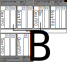
\includegraphics[width=\columnwidth]{\chapterdirectory/figure/dual_store/f07.pdf}
\caption{%
The data message moves from one core's outgoing data queue to the other's
incoming one.
}
\end{subfigure} &
\begin{subfigure}[t]{0.47\textwidth}
\includegraphics[width=\columnwidth]{\chapterdirectory/figure/dual_store/f08.pdf}
\caption{%
Upon reception of data, $C_B$ simply completes its core's request.
}
\end{subfigure}
\end{tabular}
\end{center}
\caption{Illustrations for \textbf{Parallel Stores}}
\label{fig:split_msi_dual_store}
\end{figure}
% Very simple example that must be fully illustrated to show how the FIFOs work.
\stopallthesefloats
